\documentclass[10pt,twoside, twocolumn, openany,nodeprecatedcode]{dndbook}

\usepackage[english, italian]{babel}
\usepackage[utf8]{inputenc}
\usepackage{lipsum}
\usepackage{listings}
\usepackage{flushend}
\usepackage{bookmark}
\usepackage{dblfloatfix}
\usepackage{tikz}

\usepackage{tikzpagenodes}

\lstset{%
  basicstyle=\ttfamily,
  language=[LaTeX]{TeX},
}


\begin{document}
\raggedend



\thispagestyle{empty}
 \begin{tikzpicture}[remember picture,overlay]
   \node at (current page.center) {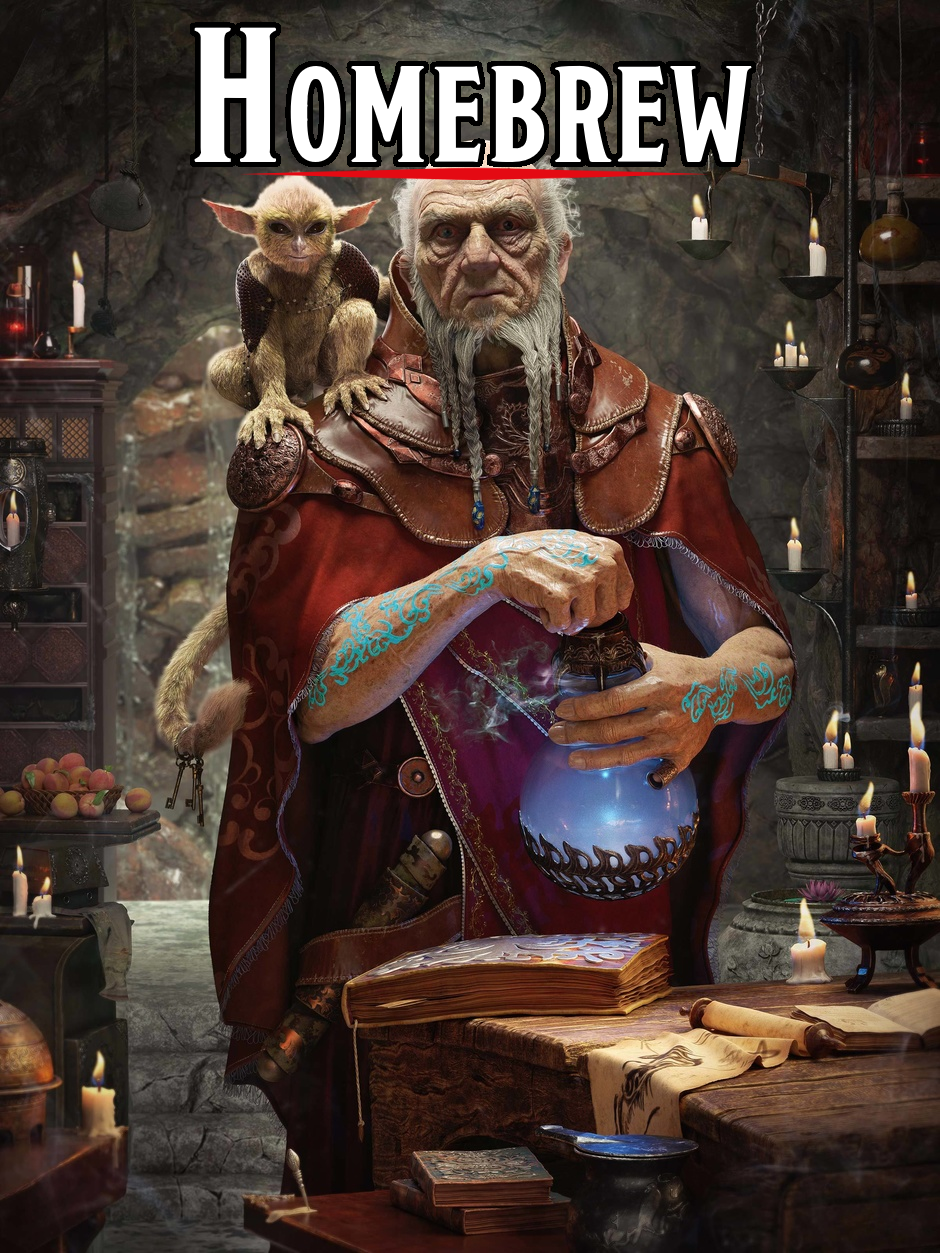
\includegraphics[width=\pdfpagewidth,height=\pdfpageheight]{0-CopertinaInizio/Risorse/backgroundTitle.png}};
 \end{tikzpicture}
\clearpage


\chapter{Struttura del Cosmo}

\section{I Piani di Esistenza}
Per comprendere come sia sbagliato parlare di posizione reciproca tra piani è necessario comprendere come le dimensioni percepite nel piano materiale, abitato da tutti noi, non sono altro che una sorta di proiezione ortogonale, su di un foglio con tre dimensioni spaziali ed una temporale, di una struttura che esiste in un ambiente infinitamente più complesso, e dove le dimensioni sono molte di più, forse infinite, e le regole della fisica che permettono alla realtà di funzionare non sono diverse, ma si comportano in modo diverso, per la diversa essenza di ciò che crediamo più familiare di quanto non sia veramente.

Tutti noi sappiamo che un grave, se non sostenuto, precipita verso il basso, attirato dal terreno, o respinto dal cosmo. Tuttavia se esistesse una direzione ortogonale a tutte e tre quelle che noi conosciamo, in cui questa forza permette un movimento, vivendo in un piano apparentemente simile al nostro (si intende qui dotato di tre direzioni spaziali ed una temporale) che condivide il tempo, una direzione verticale e la direzione verticale e la direzione accennata in precedenza al posto di una seconda direzione orizzontale, allora i gravi privi di sostegno muoverebbero naturalmente in diagonale.

Possiamo aspettarci dunque che esistano piani in cui la realtà delle cose è talmente diversa da quella che viviamo sul piano materiale, da rendere impossibile non solo la sopravvivenza, ma persino l’esistenza come esseri.

Per questo motivo, oltre che per difficoltà pratiche, il viaggio extraplanare, pur essendo, almeno teoricamente, possibile da qualunque piano ad un qualunque altro, rimane terribilmente limitato, rendendo difficile studiare la reale struttura del multiverso.

Alcuni ipotizzano persino che il multiverso, per quanto esteso ed imperscrutabile, sia solo una briciola in un oceano di multiversi, a loro volta contenuti in qualcosa di più grande e complesso.

La premessa sulla struttura multidimensionale del multiverso è necessaria per puntualizzare come è impossibile fornire una singola proiezione bidimensionale che rappresenti realisticamente la struttura dei piani conosciuti e non.

\subsection{Piani Interni: l’Etere}
I piani interni sono così detti perché l’intuizione riguardo alla loro struttura li vede come chiusi in qualche modo in una sorta di sfera, se vogliamo sperare ancora che la geometria a cui siamo abituati possa descrivere facilmente il multiverso.

Questa sfera sarebbe una sorta di ammasso di Etere, stratificato, nel quale sono sospesi i piani Interni: essa prende il nome di Piano Etereo.

Lo strato più superficiale, noto come Piano Etereo Superiore o Aether, contiene i piani Materiali, che si comportano come tante isole sospese in un mare gassoso: è possibile muoversi da un piano all’altro sia tramite portali planari che deformano il piano etereo, sia tramite, almeno teoricamente, veicoli di qualche tipo in grado di solcare l’etere come le navi solcano il mare o gli uccelli i cieli.

Tra questi piani i più degni di menzione sono Midgard (da alcuni studiosi locali chiamato anche Primo Materiale, come reminescenza dei più antichi studi del cosmo), Il Feywild e Shadowfell, ma sono solo alcuni tra i più estesi.

Più al di sotto, come un oceano di etere liquido, si estende il Piano Etereo Inferiore, o Mare dei Sogni, nella quale superficie si trovano i quattro piani elementari. È molto difficile scendere più in profondità, ma si presume che possano esistere altri piani di natura elementare, e che forse le profondità del piano etereo possano in qualche modo intersecare il piano Astrale o altre regioni ancora meno conosciute del Cosmo.

Alcuni ritengono che il Reame Remoto sfiori gli abissi del Piano Etereo, o troppo semplicisticamente persino che ne costituisca la superficie profonda.
Quest’ultima visione sottovaluta fortemente quanto aliena è l’essenza del Reame Remoto.

In realtà negli abissi più profondi del Mare dei Sogni vi sono delle creature incredibilmente antiche e lontane dalla comprensione umana: i Leviatani. Grandi a volte come interi piani di esistenza, e spesso abitati da creature mai viste da nessun abitante di Midgard, come fossero isole nascoste in un mare remoto. Per quanto apparentemente inimmaginabili queste creature sono ben lontane dagli orrori ancestrali del Reame Remoto.

Nelle più remote e impenetrabili profondità del Piano Etereo, vi è la sua superficie cristallina, forse abitata anch’essa, e forse residenza di qualche Dio, ma tutto ciò che si può dire su questa regione del multiverso è pura speculazione.
Chi sa se qualcos’altro esiste al di sotto di questo duro guscio di etere cristallizzato?

\subsection{Piani Esterni: Il Piano Astrale}
Il piano Astrale si può immaginare, secondo i modelli correnti, come una sorta di clessidra, nella quale parte alta risiedono i Piani Superiori, sede di tutto ciò che è buono, mentre nella parte bassa sono situati i Piani Inferiori, sede di ciò che è male; al suo ipotetico restringimento troveremmo l’Aether, ovvero lo strato superficiale del Piano Etereo.

Piani superiori ed inferiori sono termini che, prima di tutto, evidenziano la profonda ignoranza delle creature dei piani interni riguardo alla struttura del multiverso.

Con ogni probabilità il modello offerto non rispecchia realmente la struttura delle cose, in primo luogo perché bene e male risultano senza dubbio abbastanza arbitrari, nella loro definizione, e inoltre per la non banale assunzione del principio del terzo escluso, che non è assolutamente da dare per scontato in un universo la cui struttura ci è così oscura.

Ciò che probabilmente è vero è che per ogni piano immerso nel Piano Astrale esiste un concetto tipicamente umano associato, e un piano associato al suo contrario. Anche qui è importante notare come non sia da escludere la presenza di altri piani in qualche modo anch’essi collegati attraverso diversi impianti logici a quello “di partenza”.

La giustificazione più probabile di ciò è che siano in realtà le menti degli esseri dei piani interni ad ereditare questi concetti dalla struttura del Piano Astrale.

In realtà è più corretto pensare ai piani esistenti nel Piano Astrale come Regni. Seppur diversi tra loro come piani distinti, essi sono fortemente legati, tanto che il viaggio attraverso l’infinità del Piano Astrale risulta più semplice di molte altre forme di viaggio extraplanare (con l’eccezione della difficile impresa del lasciare il Piano Etereo).

Nei singoli regni possono esistere incarnazioni di natura divina, e possono esistere leggi fisiche e magiche anche insolitamente diverse tra loro, ma questo è quasi certamente imputabile, appunto, alla presenza di questi Dei.

\subsection{Il Reame Remoto}
È peculiare che qualcosa di così distante dai piani materiali possa essere conosciuto, e sarebbe sicuramente esagerato affermare che il Reame Remoto lo sia in alcun modo, tuttavia esso esiste, ed è percepibile.

Tutto ciò che si sa della sua natura è che è estremamente aliena: non è neppure certo che si tratti effettivamente di un solo piano, o di un piano. Ciò che si sa per certo è che si tratta di una regione tanto distorta e lontana dalla comprensione degli esseri dei piani più familiari, da sovrastare le loro menti, riempiendole di follia ed orrore, fino a distruggerle.

Casa di Intelligenze Antiche, secondo alcuni persino della Verità Assoluta (che secondo altri risiede nelle zone più remote dei Piani Superiori), esso non segue le normali leggi della logica, o forse, meglio di ogni altra parte del multiverso, dimostra come la nostra mente e i modelli che costruiamo per spiegare la realtà sono troppo semplici e limitate per arrivare alla comprensione di ciò che è.

Gli esseri ancestrali che vivono su questo piano possono a volte essere potenti quanto Dei, influenzare la realtà in modo simile, ma molto più remoto, e forse inconsapevolmente.

Potrebbero essere Dei in un altro multiverso, o in regioni talmente aliene e remote del nostro da risultare tanto incomprensibili… o forse là dove esistono hanno l’importanza di una zecca appesa ad un filo d’erba su una pozzanghera, e le infinite riflessioni della sua immagine attraverso gli strati del multiverso proiettano ombre mostruose sul nostro mondo, rendendola fonte di potere.
Probabilmente non otterremo mai una grande conoscenza del Reame Remoto, ma chi può dire con certezza che ciò è un male?

\subsection{Il Vento Cosmico}
Il Vento Cosmico è una forza primigena del multiverso, che sembra attraversare ogni cosa ed ogni istante. Esso permette di veicolare potere da un luogo all’altro dell’universo, che sia o meno sullo stesso piano.

Il vento soffia dal caos della creazione fino alla fine del cosmo, ed è il principale veicolo della magia arcana, che permette di manipolare la sostanza secondo la volontà dell’incantatore. Il Potere divino si comporta in modo simile, scorrendo nel Vento, ma provenendo da un’intelligenza più remota, che spesso non si trova neppure sullo stesso piano di esistenza dell’incantatore.

Pur scorrendo in tutto l’universo, il Vento Cosmico non percorre tutta la realtà in modo uniforme, ma filtra nei piani come aria da sotto una finestra chiusa. Per questo motivo esistono piani dove la sua presenza è maggiore, e piani dove è minore, e addirittura zone in cui è disomogeneo all’interno di uno stesso piano.
Per questo motivo la forza o persino la possibilità di realizzare incantesimi può subire influenze della sua diversa presenza.

Secondo alcuni il vento sarebbe persino la magia stessa, e degno di venerazione divina, tuttavia questa visione risulta coerente quanto l’adorazione della gravità, o di qualunque altra legge dell’universo.

\section{Lo Squarcio e L'instabilità}
\subsection{Gli Edæin}

Come noto a molti, L'umanità è una razza giovane e frenetica persino per gli standard di Midgard. Durante la loro fanciullezza gli umani erano uniti in un'unico popolo: gli Edæin.
Affacciatisi da poco in un mondo ancora selvatico, in compagnia delle più antiche e sviluppate delle razze mortali --Elfi e Nani--, gli uomini tentarono di ritagliarsi uno spazio nel mondo organizzandosi in un regno dalla efficente burocrazia e temibile potenza militare.

Provenienti dal nord del mondo, furono tra i primi a perfezionare l'uso della magia di invocazione e studiarono intensamente il suo uso a scopo militare. In generale le loro conoscenze magiche rivaleggiavano e, a volte superavano, quelle degli Elfi.

Non ci volle che qualche secolo prima che i maghi degli Edæin scoprissero il ruolo del Vento come fonte e veicolo della magia arcana e ricercassero metodi per aprire tagli nel multiverso per attingere maggiore potere.

Vennero creati alcuni artefatti che permettevano di creare minuscoli fori nella trama del piano materiale, e attingere a maggior potere, ma il loro effetto relativamente ridotto e la difficoltà nel produrli non permise di sfruttarli su larga scala per ottenere un netto vantaggio militare.

Fu durante degli esperimenti per creare aperture di maggiore dimensione che si aprì ciò che ora è conosciuto come Lo Squarcio. I maghi Edæin crearono un'imponente apertura che non furono in grado di limitare: essa sfuggì al loro controllo e provocò tagli e fratture nella struttura stessa del multiverso.
Un'imponente fonte di magia selvaggia ne scaturì con inaudita violenza, provocando la devastazione del regno ed il suo trasferimento, in pezzi, in diverse regioni del multiverso, e forse anche in zone più remote della realtà. Le coscienze di chi venne coinvolto in tale incidente si persero nel confronto con una realtà che non erano fatti per comprendere, e i loro corpi furono trasmutati dalla Magia priva di controllo.

Questo cataclisma provocò una generale instabilità del multiverso, facendo avvicinare tra loro i piani e aprendo alcune feritoie, seppur modeste, che li collegano.
Questo diede inizio, tra le altre cose, ad una guerra tra i piani superiori ed inferiori, e permise il fluire di potere divino da un piano all'altro.

Ora, nel nord, dove un tempo sorgeva il regno degli Edæin rimangono solo un cratere sterminato ed un forte vento magico, che rende impossibile per chiunque viverci. Dove sorgeva l'antica capitale, ora, solo un profondo squarcio, da cui fluiscono venti iridescenti e carichi di potere, si staglia nella desolazione.

Del popolo degli Edæin rimangono diverse comunità, fuori dal piano materiale, ormai prive di ciò che le rendeva umane. Alcune sono bloccate in bolle temporali che si ripetono all'infinito e non permettono comunicazioni con l'esterno.
Il Re e la sua guardia d'onore, insieme a parte dell'esercito sono ora entità vicine a degli spettri, ossessionate dall'invertire tale errore, ma privi del potere per farlo.
Per non precludere questa possibilità però difficilmente permetteranno a qualcuno di chiudere lo squarcio, o riportare stabilità nei piani prima di aver ripristinato il loro regno.

In una scala più ampia lo squarcio è assimilabile ad una vera e propria rottura del guscio che separava l'universo dai remoti e occulti oceani della realtà più profonda, permettendo il filtrare nei piani del multiverso locale di esseri al di là della comprensione degli abitanti di questi piani.
Non déi, ma entità misteriose e trascendenti. Sono svariati gli individui che nel multiverso mirano a trascendere l'esistenza planare e acquisire la conoscenza di queste entità, considerate da loro superiori a uomini e dei.

\clearpage
%----------------------------------------------------------------------------------------------------------------------------------------------------------------------------------------------------------------------------------------------------------------------------------------------------------------------------------------

\chapter{Capitolo 2: Razze} %----------------------------------------------------------------------------------------------------------------------------------------------------------------------------------------------------------------------------------------------------------------------------------------------------------------------------------------

\section*{Presentazione}
Si noti innanzitutto che la lista di razze qui presentate, a parte per lo Shadar-Kai e poche altre che mi riservo di aggiungere in future revisioni, riguarda prevalentemente pochi NPC unici. Ciò non offre in ogni caso una scusa per rinunciare alla loro coerenza nell'universo di gioco, e verranno pertanto trattate con la dovuta delicatezza.
 

\clearpage

\input{2-Razze/2.1-Shadar-Kai/Shadar-Kai}

\section{Fey Corgi}

\begin{figure}
   \vspace*{-3.5cm}
   %\hspace*{-2cm}
   \makebox[\textwidth][c]{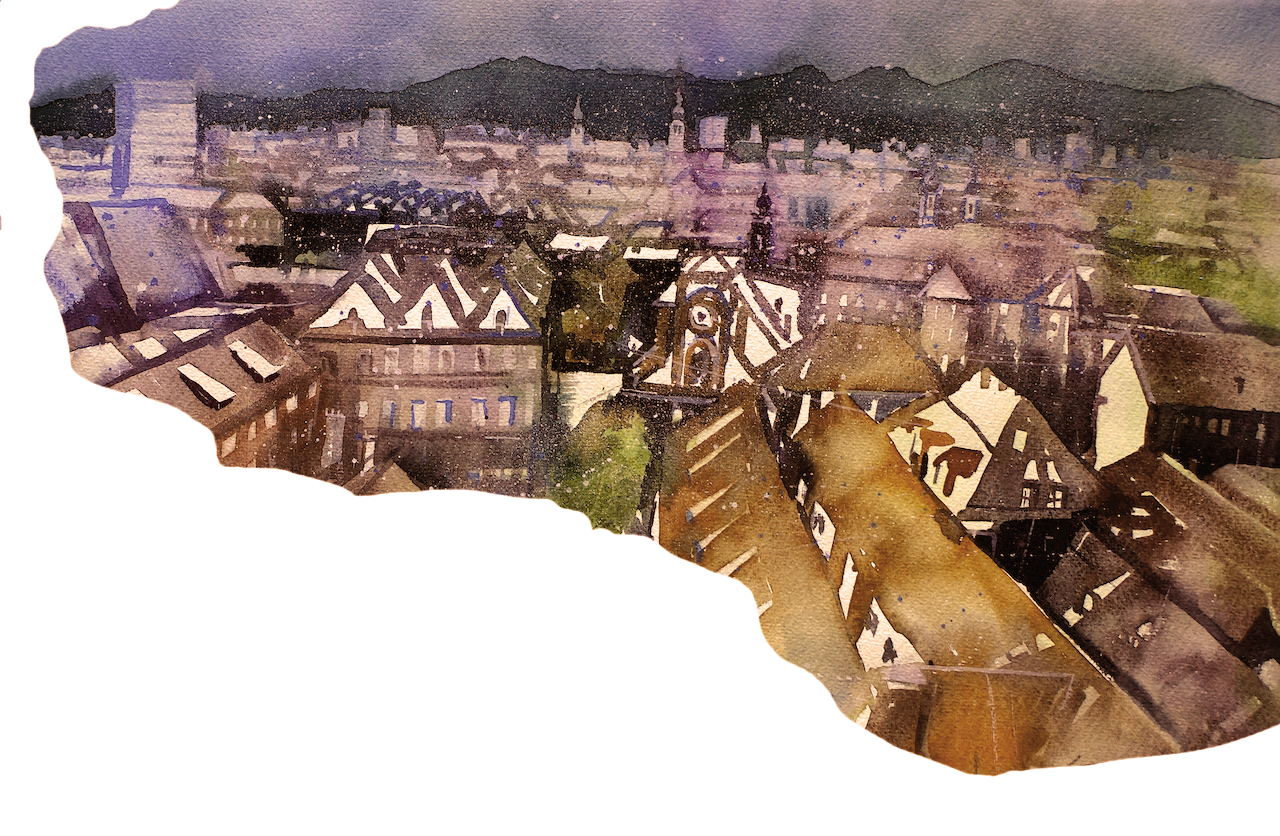
\includegraphics[width=1.1\pdfpagewidth]{2-Razze/2.2-FeyCorgi/Risorse/townbg.png}}
\end{figure}


\begin{figure}
  % \vspace*{-2cm}
   \hspace*{-10cm}
   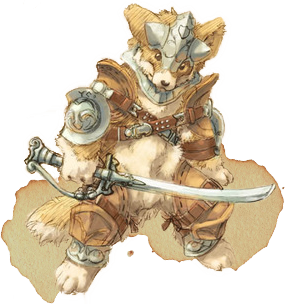
\includegraphics[width=10cm]{2-Razze/2.2-FeyCorgi/Risorse/fey_corgi2.png}
\end{figure}

\subsection{Viaggiatori dal Feywild}
I Fey Corgi sono, come intuibile dal nome, fate a tutti gli effetti. Molto rari a Midgard, vivono in piccole tribù nelle foreste del Feywild, assieme a spiriti della natura come driadi e ninfe.

La loro presenza a Midgard è lentamente cresciuta dopo lo Squarcio, ma i loro numeri sono ancora trascurabili, persino rispetto a tutte quelle creature maligne provenienti dallo stesso piano.

\subsection{Simili a Cani}
Pur dotati di un'intelligenza nettamente superiore, caratterialmente non sono dissimili dai Corgi del Primo Materiale: sono tendenzialmente amichevoli, amano stare tra la gente e si mescolano facilmente con altre culture e gruppi di altre razze intelligenti.

Sviluppano forti legami con coloro con cui passano molto tempo, anche con chi non li tratta con la dovuta gentilezza. Non è impossibile farli arrabbiare, ma è estremamente raro che finiscano per l'odiare qualcuno.

I Fey Corgi sono una specie molto curiosa, e arrivano anche a rubare e accumulare oggetti di poco valore, come calzini o biancheria: non è raro che la loro curiosità li faccia finire nei guai. Sono bassi, ma i loro sensi sviluppati li rendono ottimi avventurieri, in grado in caso anche di difendersi con i denti. Letteralmente.

\subsection{Nomi dei Fey-Corgi}
Per via della loro natura di fate i Fey Corgi sono estremamente gelosi dei loro veri nomi, per questo motivo, e per il naturale apprezzamento che hanno per i nomi dei cani delle razze di Midgard, che trovano esotici e gioiosi, tendono ad adottare semplici nomi canini:

\textit{\textbf{Nomi Maschili:}} Lucky, Rex, Spot, Rover, Buddy.

\textit{\textbf{Nomi Femminili:}} Sasha, Lucy, Bella, Lady.

\subsection{Tratti Raziali dei Fey Corgi}

In quanto Fey Corgi il tuo personaggio ha diverse capacità magiche e fisiche, dovute sia al suo retaggio fatato che canino.

\textit{\textbf{Aumento Abilità}} La tua Saggezza aumenta di 2.

\textit{\textbf{Età}} I Fey Corgi vivono un po' più dei cani comuni, e maturano un po' più lentamente. I Fey Corgi raggiungono tipicamente la maturità attorno ai due anni e tipicamente sopravvivono da 28 a 34 anni.

\textit{\textbf{Allineamento}} I Fey Corgi sono fortemente influenzati dall'ambiente sociale in cui crescono, ciononostante tendono generalmente più verso allineamenti buoni.

\textit{\textbf{Stazza}} I Fey corgi sono poco più grandi di quelli del piano materiale, aggirandosi attorno ai 3 o 4 piedi, solitamente tendenti al basso di queste misure. La tua taglia è piccola (small).

\textit{\textbf{Velocità}} I Fey Corgi sono in grado di muoversi facilmente sia a due che a quattro zampe, raggiungendo nel primo caso una velocità base di 25 piedi, e nel secondo di 35 piedi. Un Fey corgi che si muove a quattro zampe non potrà usare le zampe anteriori nel suo turno, potrà quindi attaccare solo con il morso.

\textit{\textbf{Scurovisione}} Essendo in parte cane hai una capacità superiore di vedere al buio. Vedi nella penombra come se fosse luce piena e nell'oscurità come fosse penombra entro 60 piedi. Non vedi i colori a qualunque luminosità, solo gradienti di grigio.

\textit{\textbf{Olfatto e Udito fini}} Avendo un olfatto e udito più acuti del normale sei proficente nella skill Percezione e hai vantaggio in tutti quei tiri che coinvolgono l'annusare o ascoltare.

\textit{\textbf{Natura Fatata}} Hai vantaggio sui tiri salvezza contro l'essere affascinato (charm) e non puoi essere addormentato magicamente

\textit{\textbf{Ladro-Batuffolo}} Come azione puoi compiere un attacco corpo a corpo. Se colpisci il bersaglio deve compiere un tiro salvezza sulla Forza con DC15 o essere buttato a terra (knocked prone) privo di un calzino. Questo aspetto non si applica se il bersaglio non indossa calzini. Ogni altro genere di calzatura non viene rimosso né offre protezione al calzino.

\textit{\textbf{Morso}} Puoi decidere di usare al più un attacco per turno per mordere un avversario. Esegui un attacco corpo a corpo, se colpisci infliggi 1d4+STR danni perforanti (piercing). Se vuoi puoi usare una bonus action per forzare una presa (grapple) sul tuo bersaglio. Se esegui la presa con successo l'avversario è buttato a terra (knocked prone)

\textit{\textbf{Lingue}} Sai parlare, leggere e scrivere il comune e la lingua della tua comunità. Se quella lingua è il comune, scegline pure un'altra. Puoi comunicare con i cani, tuttavia essi non hanno un vero linguaggio, e le informazioni che possono trasmettere sono minime.

\textit{\textbf{Sottorazze}} Più che in effettive sottorazze i Fey Corgi si suddividono in base alle rispettive comunità di appartenenza, che ne determinano la crescita: i Fey Corgi dei Boschi e i Fey Corgi Urbani.

\subsubsection{Fey Corgi dei Boschi}
Alcuni Fey Corgi si aggregano in piccole comunità in foreste che ricordano loro quelle del Feywild da cui provengono. Queste comunità tendono indirettamente ad attirare altra magia del Feywild, permettendo la crescita di funghi e fiori di quel piano, e attirando a volte anche Driadi e Ninfe, che apprezzano particolarmente la compagnia di questa specie.

\textit{\textbf{Aumento Abilità}} La tua destrezza aumenta di due punti.

\textit{\textbf{Maschera delle Selve}} Puoi tentare di nasconderti anche quando sei coperto leggermente da fogliame, pioggia intensa neve fitta, nebbia o altri fenomeni naturali.(Mask of the Wild)

\textit{\textbf{Addestramento nei Boschi}} Sei proficente con l'uso di Balestra leggera, balestra da braccio, arco corto, arco lungo e spada corta (hand crossbows, Longbows, Light Crossbows, Shortbows and Shortsword)

\textit{\textbf{Competenze naturali}} Sei proficente nella skill Natura (Nature).

\subsubsection{Fey Corgi Urbano}
I Fey Corgi Urbani apprezzano comunque i Boschi e la natura, ma, affascinati dalle grandi città e dalla frenesia delle razze del Primo Materiale si sono mescolati maggiormente con le culture del posto. La loro naturale curiosità li spinge a interessarsi di storia, tecnologia e tecniche rare nel Feywild.

\textit{\textbf{Aumento Abilità}} Il tuo punteggio di Intelligenza aumenta di 2.

\textit{\textbf{Interesse nell'artigianato}} Sei proficente in un attrezzo da artigiano (artisan tool) a tua scelta.

\textit{\textbf{Adorabile}} Sei competente nella Skill Persuasione (persuasion).

\textit{\textbf{Astuzia}} Sei competente nella Skill Ingannare (deception).

\begin{figure}[t]
  % \vspace*{-2cm}
  % \hspace*{-10cm}
   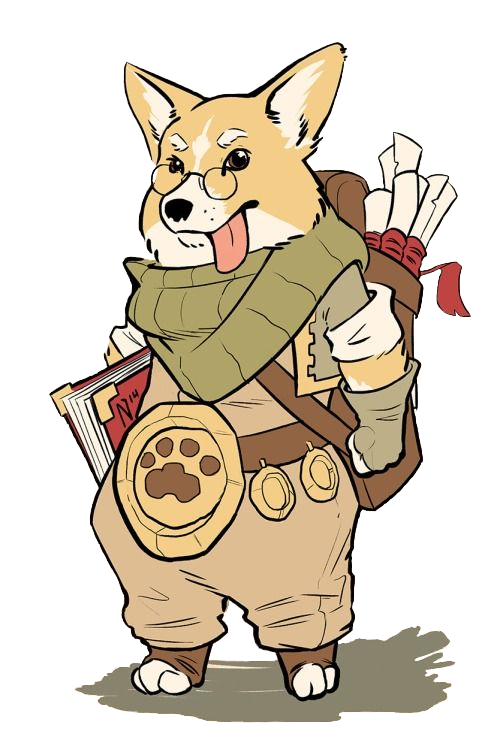
\includegraphics[height=10cm]{2-Razze/2.2-FeyCorgi/Risorse/Fey_Corgi3.png}
\end{figure}

\clearpage


\input{2-Razze/2.3-Nani/nani}

\chapter{Capitolo 3: Classi e Opzioni} %----------------------------------------------------------------------------------------------------------------------------------------------------------------------------------------------------------------------------------------------------------------------------------------------------------------------------------------
\input{3-Classi/FighterShoei}

\input{3-Classi/FighterKinsect}

\input{3-Classi/WarlockCO}


\chapter{Capitolo 4: Il Mondo di Gioco} %----------------------------------------------------------------------------------------------------------------------------------------------------------------------------------------------------------------------------------------------------------------------------------------------------------------------------------------
\input{4-Territori/Location_merger}

\chapter{Capitolo 5: NPCs} %----------------------------------------------------------------------------------------------------------------------------------------------------------------------------------------------------------------------------------------------------------------------------------------------------------------------------------------

\section{Arc Renan di Tolera}
Inventore Gnomo della città libera di Tolera. Lui e il fratello fondarono la Renan Bros Company che si occupa della produzione e distribuzione di artefatti magici minori e opere meccaniche di varia natura.

\section{Nano dei cazzotti}
Chierico nano di Huin, frequenta la regione medioccidentale del continente a cui devo ancora dare un nome. Potrebbe essere in cerca di un antico santuario nanico per restaurarlo. Lo cerca in seguito a delle voci per avviare un processo diplomatico che permetta al suo ordine di iniziare degli effettivi lavori di restauro. Questo filone potrebbe portare sulle montagne e a scontri più o meno grandi con gli orchi. Il loro popolo ha diritto di abitare le montagne? 

\section{Loran, Bastardo di Grunbaum}
Cresce con la madre, lontano dalla corte, ma ricevendo tutele e sussidi da distanze socialmente opportune. Quando la madre attacca la Gonorrea al Marchese, questo le nega il suo supporto accusandola di infedeltà. Il marchese è chiaramente sposato e sessualmente attivo con altre donne. Figures.
Comunque la madre, sfrattata e malata, non ha le possibilità economiche di mantenersi, e Loran, ai tempi adolescente, inizia a intrattenere rapporti malavitosi nel tentativo di garantire a sua madre le cure necessarie. La madre morirà in pochi mesi e Loran si ritroverà troppo legato a certi ambienti per distaccarsene.
Si darà quindi al banditismo dopo aver raccolto qualche uomo fidato durante la sua carriera criminale, anche grazie al proprio carisma.
Ora Loran è ricercato e la sua discendenza è un malcelato segreto, che corre in ogni taverna della marca. Dopo anni dall'inizio della sua \textit{carriera} è a capo di uno dei più grandi gruppi criminali della zona.

\chapter{Capitolo 6: Oggetti ed Equipaggiamenti} %----------------------------------------------------------------------------------------------------------------------------------------------------------------------------------------------------------------------------------------------------------------------------------------------------------------------------------------
\section{Oggetti per Avventurieri}
\subsection{Commodities}
\subsubsection{Mangiafuliggine}
{Wonderous item, common}

Questo è probabilmente tra i più semplici e utili oggetti magici per un avventuriero. Ha le dimensioni di una tazza con un piccolo anello che permette di appenderlo, se necessario. Alla base una sezione girevole permette di attivarlo. Una volta attivo questo oggetto raccoglie tutto il fumo nel raggio di venti piedi: non abbastanza da celare l'odore ma più che sufficente per celare colonne di fumo all'aperto o permettere l'accensione di piccoli fuochi al chiuso senza soffocare.
il fumo raccolto viene compresso e solidificato. Una volta pieno, il Mangiafuliggine deve essere svuotato o rischia di rompersi. L'autonomia è di circa una decina di ore con fuoco da campo.

\textsc{ATTENZIONE: questo prodotto è coperto da brevetto secondo le leggi Toleriane, codice 742.10/B a nome di Arc Renan di Tolera}

\input{6-Oggetti/Bozze}

\end{document}
